\documentclass{beamer}

\usepackage{wrapfig}
\usetheme{Warsaw}

\title{Augmented Reality: Technology \& Applications}
\author{Jithu Sunny}
\begin{document}


\begin{frame}
	\maketitle
	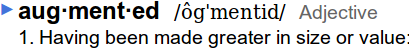
\includegraphics[scale=.5]{augmented.png}\\
	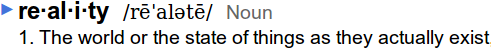
\includegraphics[scale=.5]{reality.png}
\end{frame}


\begin{frame}{What is Augmented Reality?}
\pause {\centering A Picture is worth a 1000 words..!}
	\begin{figure}
		\pause 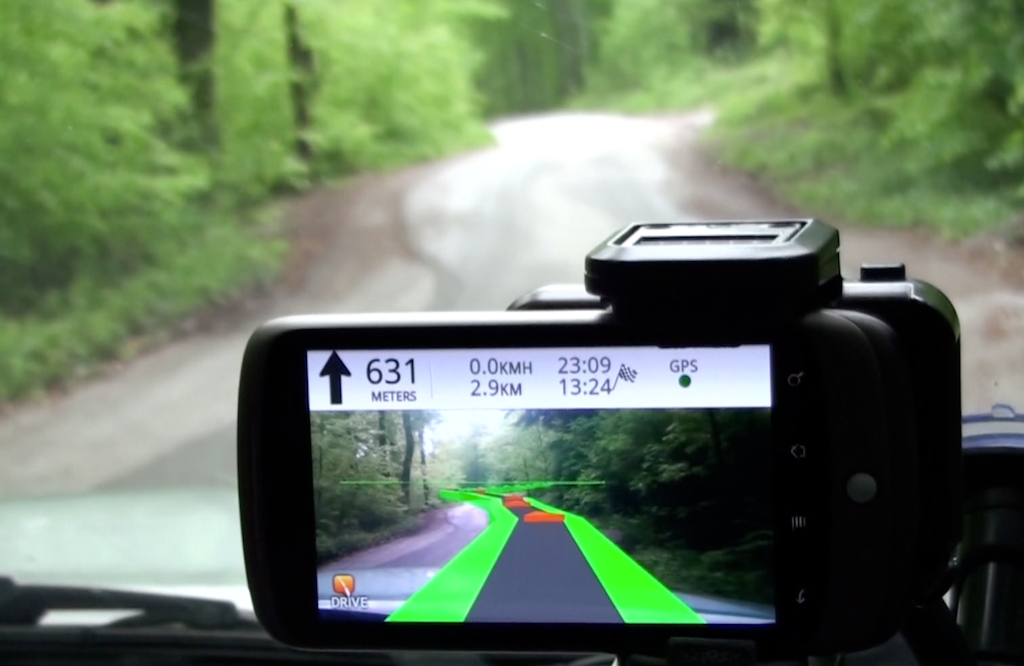
\includegraphics[scale=.25]{wikitude.png}\\
		\caption{Wikitude drive, an Augmented Reality Navigation system for smart phones.}
	\end{figure}
\end{frame}


\begin{frame}{Overview of Session}
	\begin{itemize}
		\item Introduction
		\item Hardware
		\item Software \& Algorithms
		\item A Sample Algorithm
		\item Applications
		\item Conclusion
	\end{itemize}
\end{frame}


\begin{frame}{Formal Description}
	\begin{quote}
		“Augmented reality (AR) is a term for a live direct or an indirect view of a physical, real-world environment whose elements are augmented by computer-generated sensory input such as sound, video, graphics or GPS data.”
	\end{quote}
	\begin{itemize}
		\item Artificial information about the environment and its objects can be overlaid on the real world.
		\item Enhances one’s current perception of reality. 
		\item By contrast, virtual reality replaces the real world with a simulated one.
	\end{itemize}
\end{frame}


\begin{frame}{Hardware}
- Processor, camera, display \& sensors such as accelerometer, GPS, solid state compass.\\
	\begin{itemize}
		\item Display
		\begin{itemize}
			\item HMD
			\item Handheld
			\item Spatial
		\end{itemize}
		\item Tracking 
		\item Input Devices
	\end{itemize}
\end{frame}


\begin{frame}{Display Technique}
\textbf{Head Mounted Display(HMD)}
	\begin{wrapfigure}{r}{0.5\textwidth}
  		\begin{center}
    			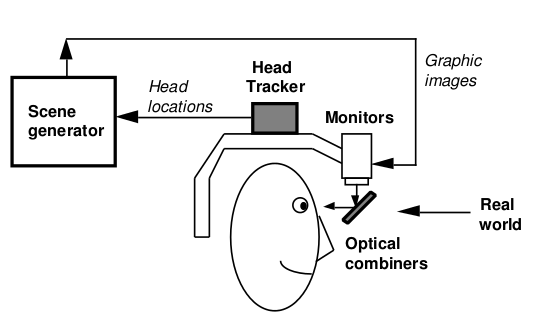
\includegraphics[width=0.48\textwidth]{hmd.png}
  		\end{center}
	\end{wrapfigure}
	\begin{itemize}
		\item Places AR over the user's view of the world.
		\item Either optical see–through or video see–through.
		\item Optical see-through employs half-silver mirrors.
		\item Increased immersive experience.
	\end{itemize}
\end{frame}


\begin{frame}{Display Techniques}
\textbf{Handheld Devices}
	\begin{wrapfigure}{r}{0.5\textwidth}
  		\begin{center}
    			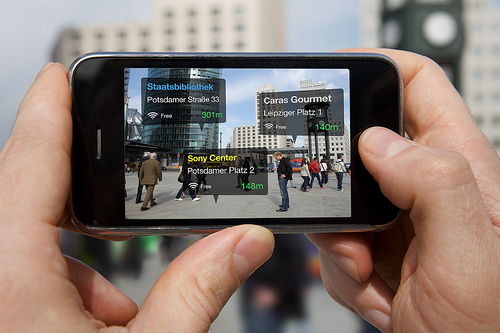
\includegraphics[width=0.48\textwidth]{handheld.jpg}
  		\end{center}
	\end{wrapfigure}
	\begin{itemize}
		\item A small display in user's hand.
		\item Apt for portability and video see-through.
		\item Disadvantage is that in most cases user has to hold the device out in front of them.
	\end{itemize}
\end{frame}


\begin{frame}{Display Techniques}
\textbf{Spatial Augmented Reality}
	\begin{itemize}
		\item Uses digital projectors to display graphical information on physical objects.
		\item The tangible nature of SAR provides the passive haptic sensation.
		\item The user is not required to carry equipment or wear the display over their eyes.
		\item This makes it a perfect candidate for collaboration.
		\item MIT-ian Pranav Mistry's Sixth sense is all about SAR.
	\end{itemize}
\end{frame}


\begin{frame}{Pranav Mistry – Sixth Sense}
	\begin{figure}
		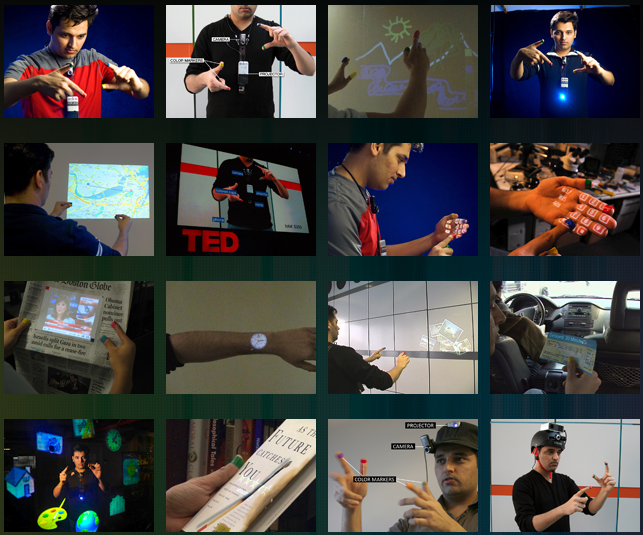
\includegraphics[scale=.37]{sixthsense.png}\\
		\caption{Pranav Mistry, Sixth Sense Technology}
	\end{figure}
\end{frame}


\begin{frame}{Tracking}
	\begin{itemize}
		\item Tracking is following.
		\item May use: Digital cameras, accelerometers, GPS, gyroscopes, compasses, RFID, wireless sensors.
		\item The users can interact with the system using Pinch gloves.
		\item In Sixth sense the finger caps is basically pinch gloves.
	\end{itemize}
\end{frame}


\begin{frame}{Dream come true..!}
	\begin{figure}
	    \pause 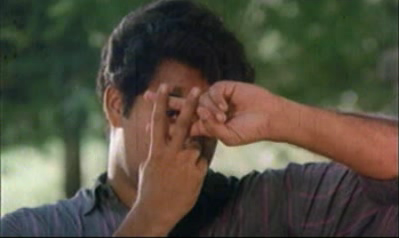
\includegraphics[scale=.3878]{mohanlal.png}
	    \pause 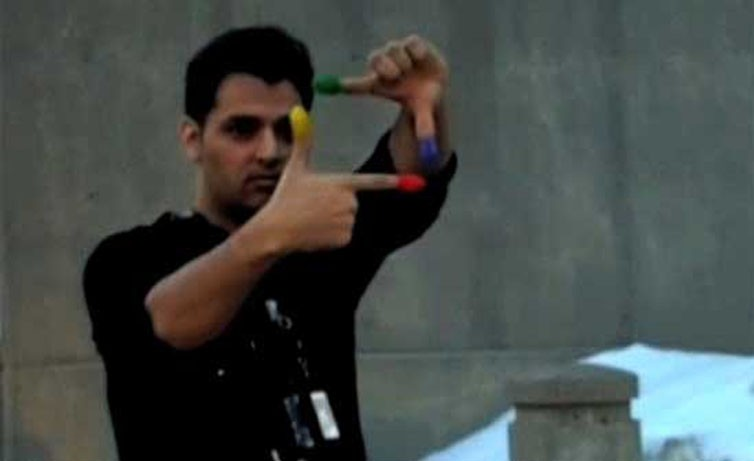
\includegraphics[scale=.20]{pranavclick.jpg}
	\end{figure}
\end{frame}


\begin{frame}{How stuff works? - Overview}
	\begin{enumerate}
		\item Capture video of the real world.
		\item Search through each video frame for markers/target object.
		\item Calculate the position of the camera relative to the marker.
		\item Draw a  computer graphics model from that position.
		\item Model is drawn on top of the video of the real world and so appears stuck on the marker.
		\item The final output is shown back in the display.
	\end{enumerate}
\end{frame}


\begin{frame}{Sample Algorithm}
	\begin{figure}
		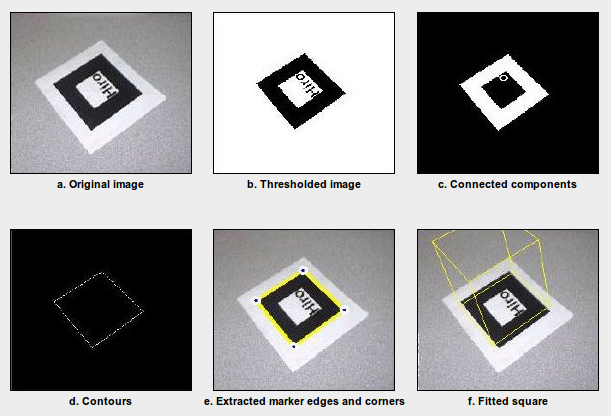
\includegraphics[scale=.50]{algorithm1.png}\\
	\end{figure}
\end{frame}


\begin{frame}{Sample Algorithm Contd.}
	\begin{figure}
		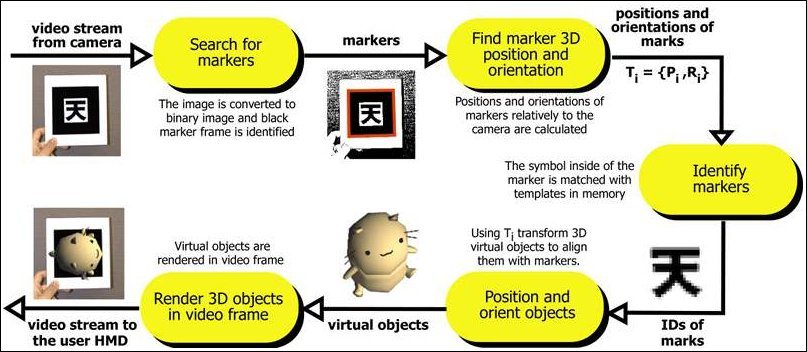
\includegraphics[scale=1.3]{flow.jpg}\\
	\end{figure}
\end{frame}


\begin{frame}{Software Toolkits}
	\begin{itemize}
		\item \textbf{ARToolKit}, an open source (dual-license: GPL, commercial) C-library to create augmented reality applications; was ported to many different languages and platforms like Android, Flash or Silverlight.
		\item \textbf{ArUco}, a minimal library for augmented reality applications based on OpenCv; licenses: BSD, Linux, Windows
mixare, Open-source (GPLv3) augmented reality engine for Android and iPhone.
		\item \textbf{OpenMAR}, Open Mobile Augmented Reality component framework for the Symbian platform, released under EPL
	\end{itemize}
\end{frame}


\begin{frame}{Applications}
	\begin{figure}
		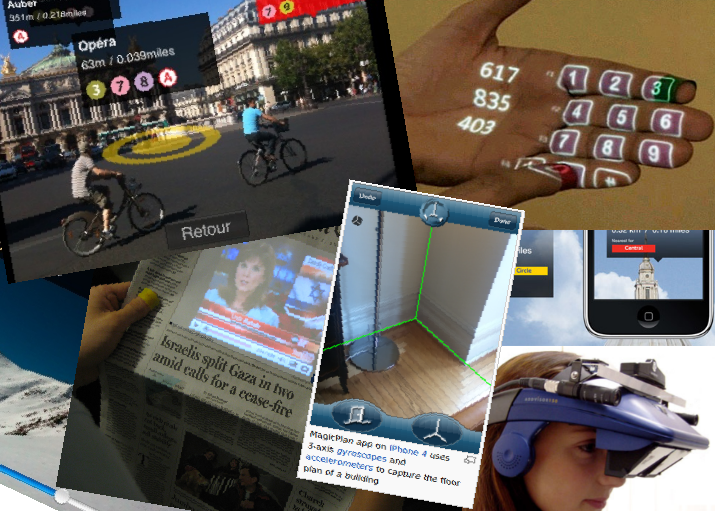
\includegraphics[scale=.40]{collage.png}\\
	\end{figure}
\end{frame}


\begin{frame}{Applications}
	\begin{itemize}
		\item \textbf{Advertising}
		\item \textbf{Task support} - Surgery, Underground pipe layout, see the fetus inside the womb..!
		\item \textbf{Navigation}
		\item \textbf{Industrial} - simulate models, reduce real time prototypes.
		\item \textbf{Military and emergency services} - provide info such as maps, enemy locations, etc.
		\item \textbf{Architecture} - simulate planned construction projects.
		\item \textbf{Entertainment and education} - virtual objects, immersive ambience, deepen the level of perception.
	\end{itemize}
\end{frame}


\begin{frame}{AR in Hollywood!}
	\begin{figure}
		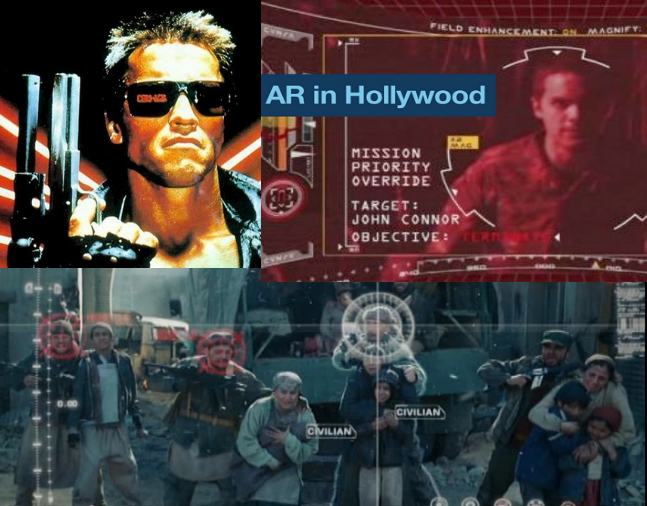
\includegraphics[scale=.45]{movie.png}
	\end{figure}
\end{frame}


\begin{frame}{Future}
	\begin{quote}
		Augmented reality has the potential to change the way we see the world in future.
	\end{quote}
	\begin{figure}
		\pause 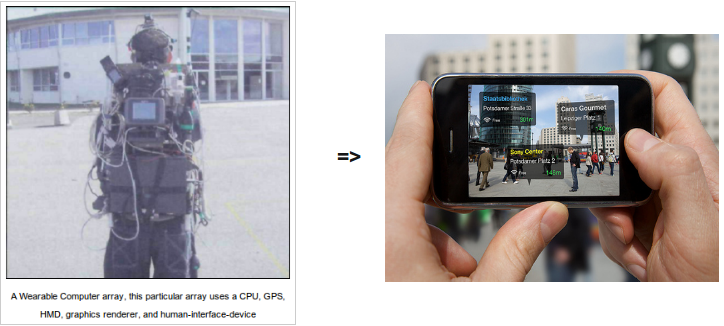
\includegraphics[scale=.45]{conclusion.png}\\
	\end{figure}
\end{frame}


\begin{frame}{Conclusion}
	\begin{itemize}
		\item Has the potential
		\item Undergoing active development.
		\item Open libraries like ARToolKit.
		\item Yet to witness applications that are so cool AND convenient. 
 	\end{itemize}
\end{frame}


\begin{frame}{References}
	\begin{itemize}
		\item ARToolKit - \emph{http://www.hitl.washington.edu/artoolkit/}
		\item Wikipedia.org - \emph{http://www.wikipedia.org/}
	\end{itemize}
\end{frame}


\begin{frame}
	\begin{figure}
		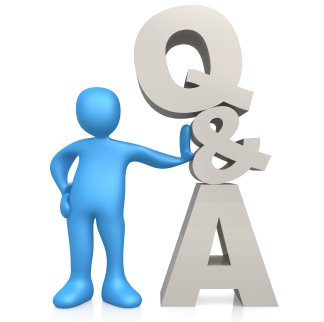
\includegraphics[scale=.70]{qa.jpg}
	\end{figure}
\end{frame}


\begin{frame}
	\begin{figure}
		
\includegraphics[scale=.60]{ty.jpg}
	\end{figure}
	\begin{center}
		\href{http://jithusunnyk.blogspot.com}{\underline{My Blog}}
	\end{center}
\end{frame}

\end{document}

